% This is "sig-alternate.tex" V2.1 April 2013
% This file should be compiled with V2.5 of "sig-alternate.cls" May 2012
%
% This example file demonstrates the use of the 'sig-alternate.cls'
% V2.5 LaTeX2e document class file. It is for those submitting
% articles to ACM Conference Proceedings WHO DO NOT WISH TO
% STRICTLY ADHERE TO THE SIGS (PUBS-BOARD-ENDORSED) STYLE.
% The 'sig-alternate.cls' file will produce a similar-looking,
% albeit, 'tighter' paper resulting in, invariably, fewer pages.
%
% ----------------------------------------------------------------------------------------------------------------
% This .tex file (and associated .cls V2.5) produces:
%       1) The Permission Statement
%       2) The Conference (location) Info information
%       3) The Copyright Line with ACM data
%       4) NO page numbers
%
% as against the acm_proc_article-sp.cls file which
% DOES NOT produce 1) thru' 3) above.
%
% Using 'sig-alternate.cls' you have control, however, from within
% the source .tex file, over both the CopyrightYear
% (defaulted to 200X) and the ACM Copyright Data
% (defaulted to X-XXXXX-XX-X/XX/XX).
% e.g.
% \CopyrightYear{2007} will cause 2007 to appear in the copyright line.
% \crdata{0-12345-67-8/90/12} will cause 0-12345-67-8/90/12 to appear in the copyright line.
%
% ---------------------------------------------------------------------------------------------------------------
% This .tex source is an example which *does* use
% the .bib file (from which the .bbl file % is produced).
% REMEMBER HOWEVER: After having produced the .bbl file,
% and prior to final submission, you *NEED* to 'insert'
% your .bbl file into your source .tex file so as to provide
% ONE 'self-contained' source file.
%
% ================= IF YOU HAVE QUESTIONS =======================
% Questions regarding the SIGS styles, SIGS policies and
% procedures, Conferences etc. should be sent to
% Adrienne Griscti (griscti@acm.org)
%
% Technical questions _only_ to
% Gerald Murray (murray@hq.acm.org)
% ===============================================================
%
% For tracking purposes - this is V2.0 - May 2012

\documentclass{sig-alternate-05-2015}


\begin{document}

% Copyright
\setcopyright{acmcopyright}
%\setcopyright{acmlicensed}
%\setcopyright{rightsretained}
%\setcopyright{usgov}
%\setcopyright{usgovmixed}
%\setcopyright{cagov}
%\setcopyright{cagovmixed}


% DOI
\doi{10.475/123_4}

% ISBN
\isbn{123-4567-24-567/08/06}

%Conference
\conferenceinfo{PLDI '13}{June 16--19, 2013, Seattle, WA, USA}

\acmPrice{\$15.00}

%
% --- Author Metadata here ---
\conferenceinfo{WOODSTOCK}{'97 El Paso, Texas USA}
%\CopyrightYear{2007} % Allows default copyright year (20XX) to be over-ridden - IF NEED BE.
%\crdata{0-12345-67-8/90/01}  % Allows default copyright data (0-89791-88-6/97/05) to be over-ridden - IF NEED BE.
% --- End of Author Metadata ---

\title{Ease the Process of Machine Learning with Dataflow}
\subtitle{[Extended Abstract]
\titlenote{A full version of this paper is available as
\textit{Author's Guide to Preparing ACM SIG Proceedings Using
\LaTeX$2_\epsilon$\ and BibTeX} at
\texttt{www.acm.org/eaddress.htm}}}
%
% You need the command \numberofauthors to handle the 'placement
% and alignment' of the authors beneath the title.
%
% For aesthetic reasons, we recommend 'three authors at a time'
% i.e. three 'name/affiliation blocks' be placed beneath the title.
%
% NOTE: You are NOT restricted in how many 'rows' of
% "name/affiliations" may appear. We just ask that you restrict
% the number of 'columns' to three.
%
% Because of the available 'opening page real-estate'
% we ask you to refrain from putting more than six authors
% (two rows with three columns) beneath the article title.
% More than six makes the first-page appear very cluttered indeed.
%
% Use the \alignauthor commands to handle the names
% and affiliations for an 'aesthetic maximum' of six authors.
% Add names, affiliations, addresses for
% the seventh etc. author(s) as the argument for the
% \additionalauthors command.
% These 'additional authors' will be output/set for you
% without further effort on your part as the last section in
% the body of your article BEFORE References or any Appendices.

\numberofauthors{8} %  in this sample file, there are a *total*
% of EIGHT authors. SIX appear on the 'first-page' (for formatting
% reasons) and the remaining two appear in the \additionalauthors section.
%
\author{
% You can go ahead and credit any number of authors here,
% e.g. one 'row of three' or two rows (consisting of one row of three
% and a second row of one, two or three).
%
% The command \alignauthor (no curly braces needed) should
% precede each author name, affiliation/snail-mail address and
% e-mail address. Additionally, tag each line of
% affiliation/address with \affaddr, and tag the
% e-mail address with \email.
%
% 1st. author
\alignauthor
Ben Trovato\titlenote{Dr.~Trovato insisted his name be first.}\\
       \affaddr{Institute for Clarity in Documentation}\\
       \affaddr{1932 Wallamaloo Lane}\\
       \affaddr{Wallamaloo, New Zealand}\\
       \email{trovato@corporation.com}
% 2nd. author
\alignauthor
G.K.M. Tobin\titlenote{The secretary disavows
any knowledge of this author's actions.}\\
       \affaddr{Institute for Clarity in Documentation}\\
       \affaddr{P.O. Box 1212}\\
       \affaddr{Dublin, Ohio 43017-6221}\\
       \email{webmaster@marysville-ohio.com}
% 3rd. author
\alignauthor Lars Th{\o}rv{\"a}ld\titlenote{This author is the
one who did all the really hard work.}\\
       \affaddr{The Th{\o}rv{\"a}ld Group}\\
       \affaddr{1 Th{\o}rv{\"a}ld Circle}\\
       \affaddr{Hekla, Iceland}\\
       \email{larst@affiliation.org}
\and  % use '\and' if you need 'another row' of author names
% 4th. author
\alignauthor Lawrence P. Leipuner\\
       \affaddr{Brookhaven Laboratories}\\
       \affaddr{Brookhaven National Lab}\\
       \affaddr{P.O. Box 5000}\\
       \email{lleipuner@researchlabs.org}
% 5th. author
\alignauthor Sean Fogarty\\
       \affaddr{NASA Ames Research Center}\\
       \affaddr{Moffett Field}\\
       \affaddr{California 94035}\\
       \email{fogartys@amesres.org}
% 6th. author
\alignauthor Charles Palmer\\
       \affaddr{Palmer Research Laboratories}\\
       \affaddr{8600 Datapoint Drive}\\
       \affaddr{San Antonio, Texas 78229}\\
       \email{cpalmer@prl.com}
}
% There's nothing stopping you putting the seventh, eighth, etc.
% author on the opening page (as the 'third row') but we ask,
% for aesthetic reasons that you place these 'additional authors'
% in the \additional authors block, viz.
\additionalauthors{Additional authors: John Smith (The Th{\o}rv{\"a}ld Group,
email: {\texttt{jsmith@affiliation.org}}) and Julius P.~Kumquat
(The Kumquat Consortium, email: {\texttt{jpkumquat@consortium.net}}).}
\date{30 July 1999}
% Just remember to make sure that the TOTAL number of authors
% is the number that will appear on the first page PLUS the
% number that will appear in the \additionalauthors section.

\maketitle
\begin{abstract}
Big data processing and machine learning have made the world a better place. However, configuring machine learning task is always a complicated job. Our system aimed to make machine learning task easy. It's a GUI-based platform designed on distributed system for big data analysis and mining. In the system, tasks are formulated by dataflow, resources are highly reusable, heterogeneous programs are mix-runnable. Meanwhile, based on Hadoop and Spark, the system is able to process massive datasets.

\end{abstract}


%
% The code below should be generated by the tool at
% http://dl.acm.org/ccs.cfm
% Please copy and paste the code instead of the example below. 
%
\begin{CCSXML}
<ccs2012>
 <concept>
  <concept_id>10010520.10010553.10010562</concept_id>
  <concept_desc>Computer systems organization~Embedded systems</concept_desc>
  <concept_significance>500</concept_significance>
 </concept>
 <concept>
  <concept_id>10010520.10010575.10010755</concept_id>
  <concept_desc>Computer systems organization~Redundancy</concept_desc>
  <concept_significance>300</concept_significance>
 </concept>
 <concept>
  <concept_id>10010520.10010553.10010554</concept_id>
  <concept_desc>Computer systems organization~Robotics</concept_desc>
  <concept_significance>100</concept_significance>
 </concept>
 <concept>
  <concept_id>10003033.10003083.10003095</concept_id>
  <concept_desc>Networks~Network reliability</concept_desc>
  <concept_significance>100</concept_significance>
 </concept>
</ccs2012>  
\end{CCSXML}

\ccsdesc[500]{Computer systems organization~Embedded systems}
\ccsdesc[300]{Computer systems organization~Redundancy}
\ccsdesc{Computer systems organization~Robotics}
\ccsdesc[100]{Networks~Network reliability}


%
% End generated code
%

%
%  Use this command to print the description
%
\printccsdesc

% We no longer use \terms command
%\terms{Theory}

\keywords{Data Mining; Big Data Analysis; Machine Learning}

\section{Introduction}
Data mining and analysis have been widely used in many industry verticals, such as financial services, communications, retails and e-commerces. However, configuring and going through the whole roadmap of data mining and analysis will be a complicated job. Integrated applications that facilitate going through the data mining and analysis job are widely demanded for data scientists and business analysts. 

Traditional tools like SAS, SPSS show their strength on descriptive and diagnostic analytics, and are useful for static structural datasets. However, they are not cloud-based, which limited the usage of advanced techniques in distributed systems. 

Aimed to facilitate data mining and analysis job, and apply machine learning to big data, we implements a modern cloud-based big data analysis system.

 Tasks in our system are formulated by GUI-based dataflow framework, that will be easy to create and understand. Also, resources like programs, datasets, job schemas and output results are highly reusable in our system. Besides, our system support heterogeneous programs, which are different languages and standalone or distributed, run together in the same job. In addition, the system is designed on distributed system, Hadoop and Spark, and choose Oozie as job scheduler, so that the system's scalability and performance is guaranteed.

In following sections, we first introduce the system overview and then explains our system main features. Finally, we give the demonstration plan.
\section{System Overview}
\subsection{System Architecture}
Our system is a GUI-based platform designed on distributed system. Figure~\ref{fig:arch} shows the architecture.

\begin{figure}[!htb]
\centering
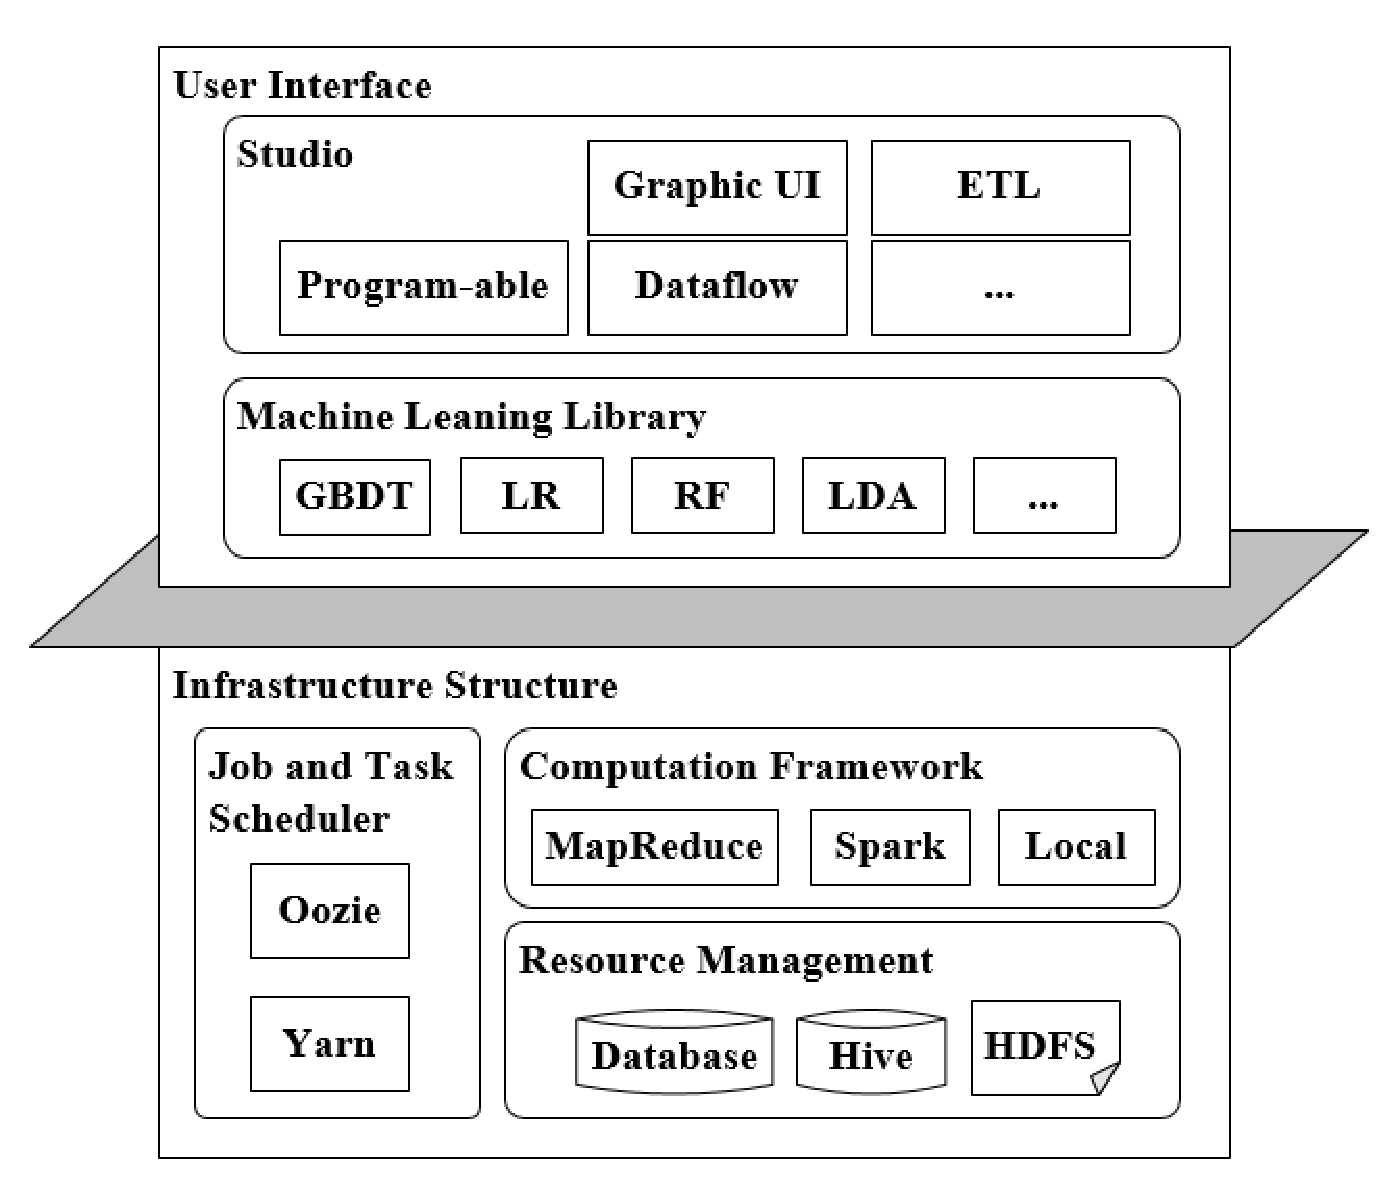
\includegraphics[height=2.8in]{arch.eps}
\caption{ An overview of system architecture.}
\label{fig:arch}
\end{figure}

The architecture is divided into two hierarchies: Infrastructure Structure Layer and User Interface Layer.
\begin{itemize}
\item \textbf{Infrastructure Structure Layer:} We use database to store meta data of programs and jobs, while other resources are stored on HDFS or managed by Hive. Jobs are scheduled by Oozie. Spark and Map-Reduce are our foundation of distributed computation framework.
\item \textbf{User Interface Layer:} This layer focuses how to provide friendly functionality for data scientists. There are two components, GUI-based Studio, Machine Learning Library.
\end{itemize}


\subsection{GUI-based Studio}
Studio is a GUI-based web service on the top of our system architecture. One must register on Studio, before using our system. Studio provides services like job creation, job management, program and dataset upload and management, and account management. It cooperates with Hadoop, Spark and Oozie that allowed data scientists to access to resources and services provided by our system easily.

It's a client of Hadoop, Spark, and Oozie services. When a job is created, it will create job's application path on HDFS, and sent job to Oozie for scheduling and run it on cloud-side finally. A job in our system denotes an unit of machine learning task, and is allowed to edit and rerun.

Although Studio provides powerful functionalities, it's emphasized that Studio is light, scalable and easy to deploy, cause it only need a database like mysql, a web server like tomcat and some configurations of Hadoop, Spark and Oozie.


\subsection{Machine Learning Library}
Machine Learning Library(ML Lib) is the algorithm library of our system, it provides a wealth of machine learning, data mining algorithms that could be categorized as pre-processing, transformation, machine learning, and evaluation. We have both Standalone and Spark implementations for each algorithm. Also, we provide a sort of API for ML Lib. 

All these algorithms are wrap as runnable programs and uploaded to our system. The runnable programs uploaded are displayed as program components of our system that are reusable. When using the algorithm, one need only click to add the corresponding component. In this way, the user is free to programming, that makes algorithms more easy use. Besides, our system allows registers to upload custom programs and third party programs to our system as well. This is different from traditional tools that are forbidden program upload.


\section{Dataflow DAG}
Before we discuss this section, let us make some clarification about workflow and dataflow.

\begin{itemize}
\item \textbf{Workflow:} is a collection of actions arranged in a control dependency DAG(Directed Acyclic Graph). Control dependency from one action to another means that the second action can't run until the first action has completed.
\item \textbf{Dataflow:} is a collection of actions arrange in a data dependency DAG, where different actions may have several different data dependency.
\end{itemize}

The concept dataflow differed with workflow as to dataflow specify data dependency between different actions. And the control dependency of actions are determined by the data dependency.

\subsection{Machine Learning Task is A Dataflow}
The bulk of the machine learning job workload consists of sequences of procedures written using a variety of tools and languages. Specifically, the control dependency of these diverse procedures could be formulated by workflow correctly. In this way, the details of procedures in the process is not concerned. While, the control dependency of procedures is underlined. 

There exists some workflow systems, such as Oozie, Azkaban. However, input and output data locations of each actions must be configured by user in those systems before it was submitted, otherwise it will failed. This implied that user have to know about where data was or will be stored. However, we believe it's not major concern users should focus on, but what the source data  how to construct the tasks and how about the results. 

Exactly, dataflow formulation of machine learning task is better, since the data dependency between actions determined the control dependency and the storage concern is eliminated in this way. 

\subsection{Dataflow with Graphical User Interface}
\begin{figure}[!htb]
\centering
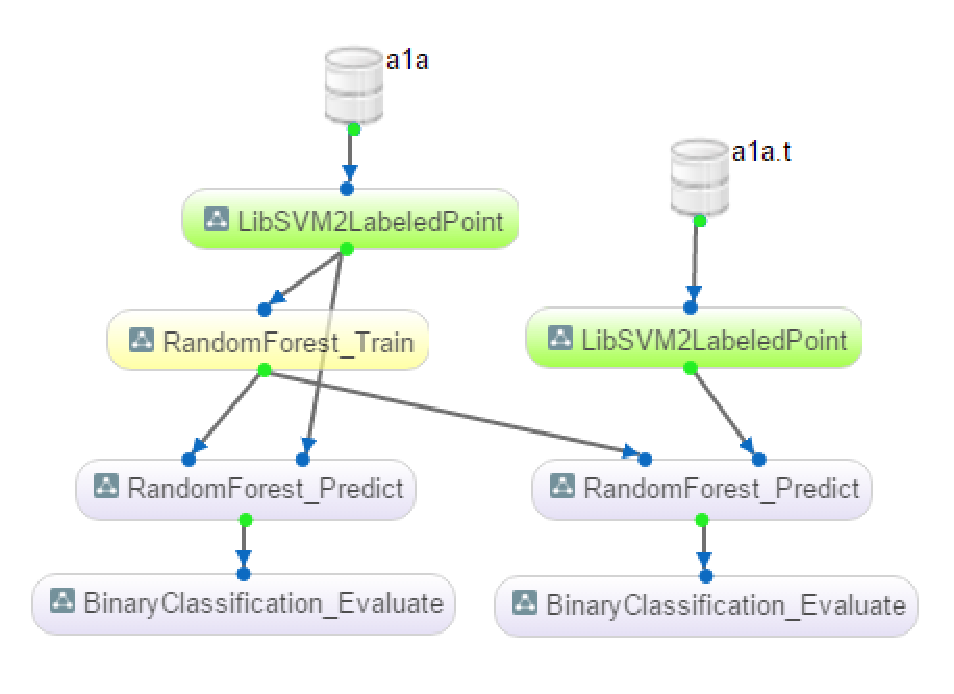
\includegraphics[height=2in]{dataflow_DAG.eps}
\caption{An example of dataflow DAG}
\label{fig:dag}
\end{figure}

We introduced GUI based dataflow DAG into our system founded on Oozie workflow. Figure~\ref{fig:dag} is an example of dataflow DAG, where each datasets and programs are displayed as GUI components.The node shape on the top of GUI components are regard as input data anchors of the program, while the node shape on the bottom are output anchors.  And the unique random HDFS file path will be generated for intermediate output data when the job is submitted. Each arrow means a dataflow between components. And arrow couldn't be linked except the anchors are type matched. After submitting a job to the cloud, each node in the job will be scheduled to execute according to the dataflow DAG. 

Based on GUI, we support user to create, configure, submit, and monitor a job in drag-and-drop manner. Also, we provide real time action state reports with color display on GUI components, where yellow, green and red mean actions is running, finished and error respectively.

\section{Advantages}
Our system has devoted to provide powerful and light solution for machine learning tasks. And it has many advantages compared to traditional tools, such as enable to process massive data, high scalability and performance etc. Beyond that, we are going to introduce some main advantages of our system.
\subsection{Lowing the Barriers}
A machine learning job is formulated as GUI-based dataflow in our system. Datasets and Programs are displayed as GUI components as well. Users are enable to create, configure, submit, and monitor a job in drag-and-drop manner. Users could track the status of job according to the state reported by dataflow DAG at runtime. The workload of workflow configurations is replaced with dataflow drawing. The implementation details of programs and the diversity of programs are hidden, while the usage are emphasized. Besides, job schema could be save, modify and reuse. In this way, machine learning is no longer a tough task. It's easy to understand and create a job in our system. Our system has lowered the barrier of machine learning.

\subsection{Highly Reusable}
As is shown above, Studio has managed a lot of resources, include dataset, program, job schema, intermediate output data. And we have done effort to make these resources to obtain fully utilized, which is approved to improve our system's user experience.

Reusability is highly supported in different aspects and granularity by our system.  Correspondingly, we have datasets and program reuse, job schema reuse and intermediate output data reuse.

The datasets and programs could be shared across different users, so that one may not need to upload a new program or dataset if there exists one in our system. Although, it is never mind to exists several program for the same algorithm, that gives user more choices and help select out the one better. 

The job schema is a XML document defines the elements, parameters and types that represent a job in our system. With job schema, it is easily to save, modify, reload and reuse a job. When the job finished error or one need to modify the job, it is not necessary to create a job new. One could directly open the old job and modify, then rerun it. Accordingly, the job schema will be update after the job is edited, while the old one be backed. We also support url get request for job, so that one could share and access to a job easily. In addition, jobs are enable to be clone that greatly facilitate who want to construct several similar jobs.

Intermediate output data is also reuse in our system. The same input and parameters for the same program will generate the same result( without randomness). It's not required to run every time even if the program has random. Therefore, it would reduce running time and save computation and storage greatly with reuse of intermediate output data. We support intermediate output data save and download functions. When a job is modify, we intelligently analysis whether actions in the job should be rerun according to actions' configuration. If the rerun actions will reuse the intermediate output data of non-rerun ones.


\subsection{Heterogeneous System Architecture}

As we all known, machine learning task always contains several procedures, such as ETL, feature engineering, and model training and evaluation. Usually, totally different programs or tools would be applied in those procedures. Those programs or tools might be implemented in different languages and run in different manners( Standalone or Distributed, Map-Reduce or Spark etc.) appropriately. 

Fortunately, machine learning procedures are regarded as data transformation in dataflow framework. That's machine learning procedures are black boxes communication with data flows. And it's never mind that procedures are heterogeneous.

There is no worry about heterogeneous programs run together in our system. Because all resources are persist on HDFS or managed by Hive in our system. We just only to focus on the problem how to access to resources on distributed system for standalone programs or tools. And our approach of the problem is fairly simple. That's we will download the resources demanded for the standalone program before start up it and then upload the result outputs after it finished.

In our system, we support tools of different languages run together, includes C/C++, Java, Scala, python, shell etc. In this way, the program uploaded to our system won't be limited by which language it implemented with. That gives user more unrestrained choices.

Moreover, we also support standalone and distributed programs run together. For some small dataset, standalone programs might be more time saving and less resource consuming. While, distributed programs have advantages in processing massive data. Hence, with the correct combinations of programs, our system will leverage their advantages.

\section{Conclusions}
This paragraph will end the body of this sample document.
Remember that you might still have Acknowledgments or
Appendices; brief samples of these
follow.  There is still the Bibliography to deal with; and
we will make a disclaimer about that here: with the exception
of the reference to the \LaTeX\ book, the citations in
this paper are to articles which have nothing to
do with the present subject and are used as
examples only.
%\end{document}  % This is where a 'short' article might terminate

%ACKNOWLEDGMENTS are optional
\section{Acknowledgments}
This section is optional; it is a location for you
to acknowledge grants, funding, editing assistance and
what have you.  In the present case, for example, the
authors would like to thank Gerald Murray of ACM for
his help in codifying this \textit{Author's Guide}
and the \textbf{.cls} and \textbf{.tex} files that it describes.

%APPENDICES are optional
%\balancecolumns
\appendix
%Appendix A
\section{Headings in Appendices}

\end{document}
